\documentclass[tikz]{standalone}
\usepackage{tikz}
\usetikzlibrary{matrix,fit,backgrounds,calc,decorations.markings,arrows.meta,shapes.geometric}
\usepackage{amsmath}
\usepackage{braket}

\begin{document}
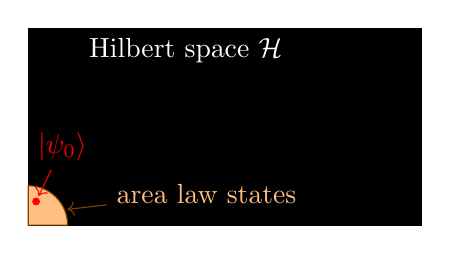
\begin{tikzpicture}
	\draw[fill=black] (0,0) rectangle (5,2.5);
	\node[below,color=white] at (2,2.5) {Hilbert space $\mathcal{H}$};
	\filldraw[fill=orange!50!white, draw=orange!50!black] (0,0) -- (0.5,0)
		arc [start angle=0,end angle=90,radius=0.5] -- cycle;
	\node[right,color=orange!50!white] (al) at (1,0.4) {area law states} ;
	\draw[->,color=orange!50!black] (al) -- (0.5,0.2);
	\coordinate (psi) at (0.1,0.3) ;
	\fill[color=red] (psi) circle [radius=0.05] ;
	\node[right,color=red] (psi_lbl) at (0.0,1) {$\ket{\psi_0}$};
	\draw[->,color=red] (psi_lbl) -- ($(psi_lbl)!0.9!(psi)$) ;
	%     \shade[ball color=black!30!white] (\i, 0) circle [radius=0.3] ;
	% % \draw[->] (0, 0) -- (5., 0) ;
	% \foreach \i in {0,...,5} {
	%     \shade[ball color=black!30!white] (\i, 0) circle [radius=0.3] ;
	%     % \draw[fill=black!30!white] (\i, 0) circle [radius=0.3] ;
	% }
	% \draw[thin,dashed,red]    (2.5,-0.5) -- (2.5,1.0);
	% \node[above,red,left]  at (2.5, 0.7) {A};
	% \node[above,red,right] at (2.5,0.7) {B};
\end{tikzpicture}
\end{document}
